%% For ACM ADAPT DL proceedings %%
\documentclass[10pt,onecolumn]{article}

\usepackage[lmargin=1in,rmargin=1in,tmargin=1in,bmargin=1in]{geometry}
\usepackage{epsfig}
\usepackage{graphicx}
\usepackage{caption}
\usepackage{subcaption}
\usepackage{float}
\usepackage{enumerate}
\usepackage{url}
\usepackage{hyperref}

\newenvironment{packed_itemize}{
\begin{itemize}
  \setlength{\itemsep}{1pt}
  \setlength{\parskip}{0pt}
  \setlength{\parsep}{0pt}
}{\end{itemize}}

\date{}

\begin{document}

\title{Introducing 1\textsuperscript{st} ACM SIGARCH ReQuEST Workshop/Tournament \\
on Reproducible Software/Hardware Co-design \\
of Pareto-Efficient Image Classification\\[.5cm]
\textbf{\href{http://cKnowledge.org/request-cfp-asplos2018.html}{cKnowledge.org/request-cfp-asplos2018.html}}
\textbf{\href{http://cKnowledge.org/request}{cKnowledge.org/request}}
}

\author{}

\maketitle
\thispagestyle{empty}
\pagestyle{empty}

\begin{center}
co-located with ACM ASPLOS 2018 (Williamsburg, VA, USA) \\
March 24th, 2018 \\
(proposal submitted in June 2017)
\end{center}

\textbf{Organizers (A-Z):}

\begin{packed_itemize}

 \item Luis Ceze, University of Washington, USA
 \item Natalie Enright Jerger, University of Toronto, Canada
 \item Babak Falsafi, EPFL, Switzerland
 \item \textit{Grigori Fursin, cTuning foundation, France (reproducibility and common workflow framework)}
 \item \textit{Anton Lokhmotov, dividiti, UK (industrial relations)}
 \item \textit{Thierry Moreau, University of Washington, USA (workshop organization)}
 \item Adrian Sampson, Cornell University, USA
 \item Phillip Stanley Marbell, University of Cambridge, UK 

\end{packed_itemize}

\textbf{Advisory board (A-Z):}

\begin{packed_itemize}

 \item Michaela Blott, Xilinx
 \item Unmesh Bordoloi, General Motors
 \item Ofer Dekel, Microsoft
 \item Maria Girone, CERN openlab
 \item Wayne Graves, ACM
 \item Vinod Grover, NVIDIA
 \item Sumit Gupta, IBM
 \item James Hetherington, Alan Turing Institute
 \item Steve Keckler, NVIDIA
 \item Wei Li, Intel
 \item Colin Osborne, ARM
 \item Andrew Putnam, Microsoft
 \item Boris Shulkin, Magna
 \item Greg Stoner, AMD
 \item Alex Wade, Chan Zuckerberg Initiative
 \item Peng Wu, Huawei
 \item Cliff Young, Google 

\end{packed_itemize}

%%%%%%%%%%%%%%%%%%%%%%%%%%%%%%%%%%%%%%%%%%%%%%%%%%%%%%%%%%%%%%%%%%%%%%%%%%%%%%%%%%%%%%%%%%%%%%%%%
\newpage

\section*{Introduction}
\label{sec:intro}

\begin{figure*}[ht]
  \centering
  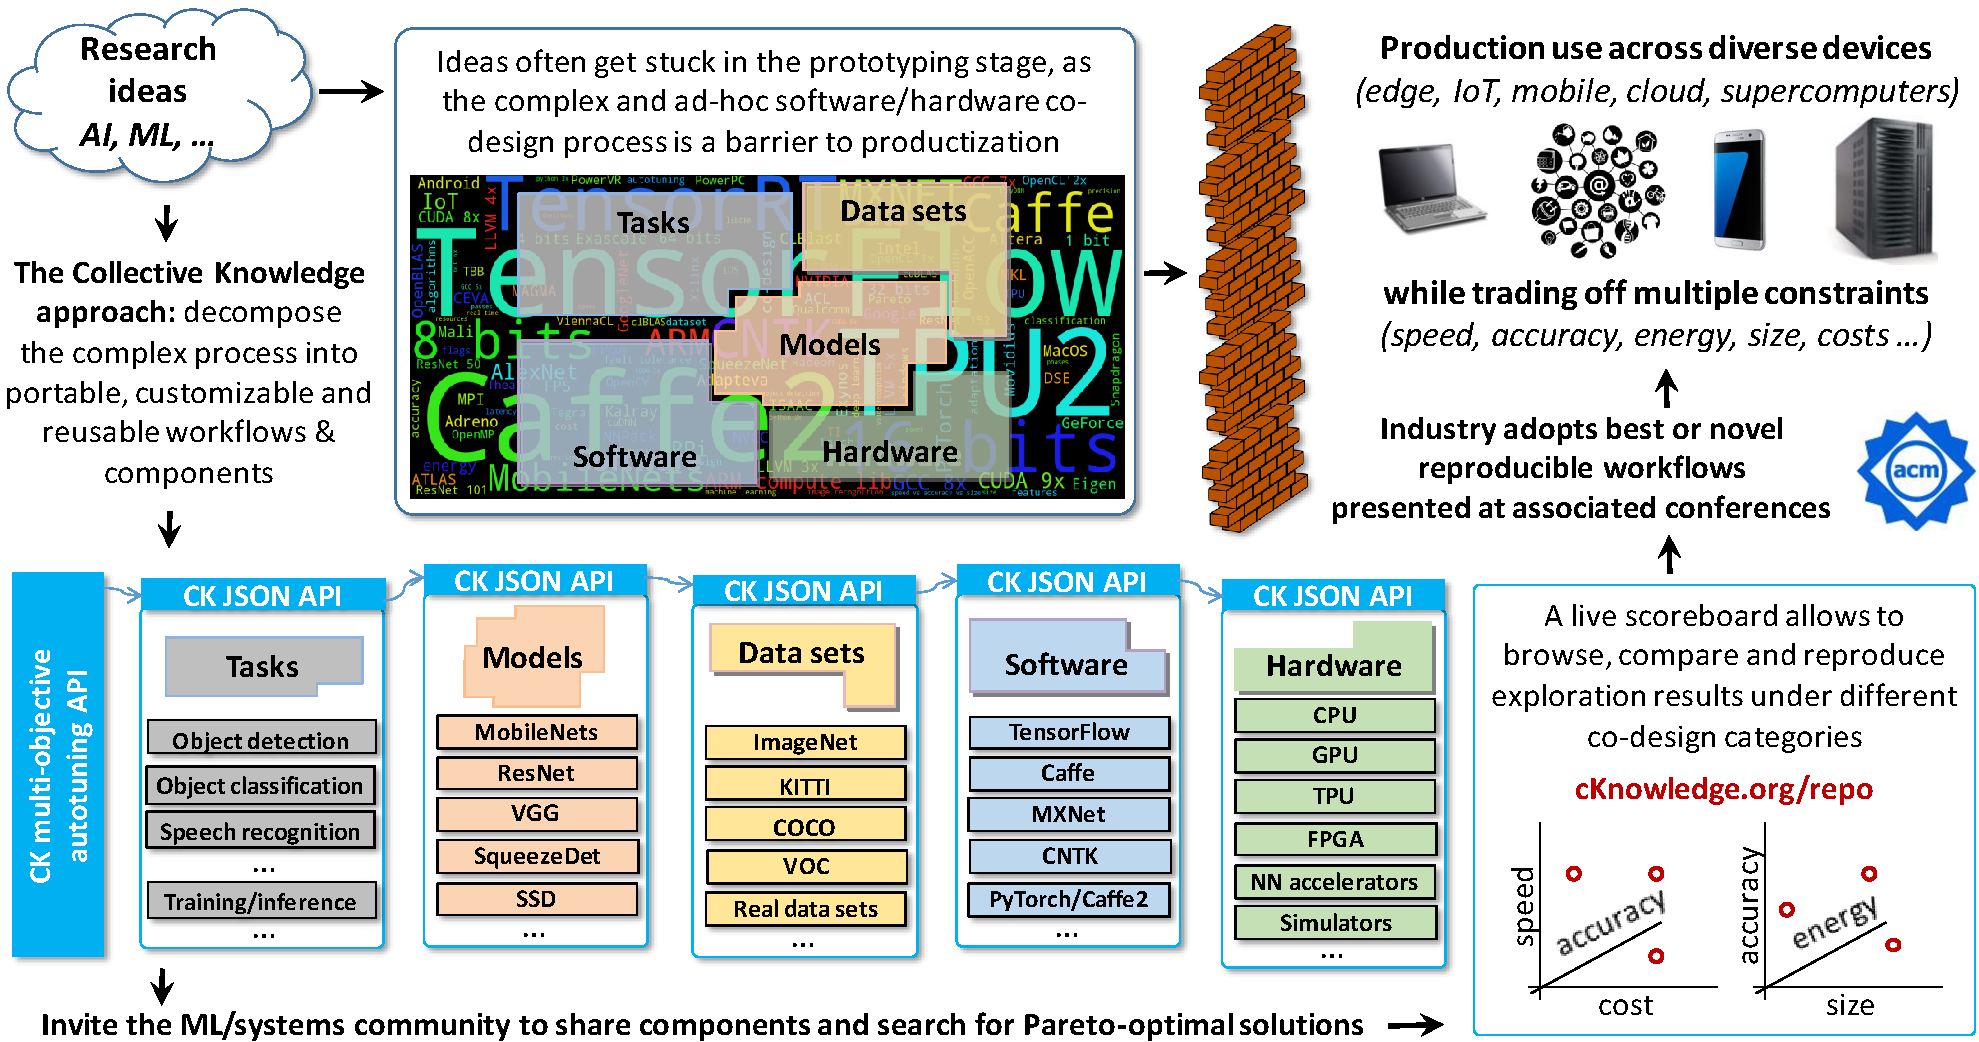
\includegraphics[width=0.9\textwidth]{figures/ck-request-concept-cropped.pdf}
  \caption{Reproducible ACM ReQuEST tournaments involving interdisciplinary community
  to decompose complex software/hardware benchmarking,
  optimization and co-design process into customizable
  Collective Knowledge workflows with reusable components, and collaboratively
  explore Pareto-efficient solutions in terms of speed,
  accuracy, energy, costs and other extensible metrics
  across diverse models, data sets, frameworks, libraries and platforms.}
  \label{fig:ck-request-concept}
\end{figure*}




\end{document}
